\chapter{apperatet}\label{ch:apperatet}
\section{apperatet}
Hørerapperatet er som beskrevet i afsnit \ref{ch:Teori} bestående af båndpas-filtre. Der opdeler input-signalet i frekvensbånd, der bliver vægtet forskelligt før de bliver sat sammen til et output-signal.

Der er blevet lavet et Matlab program, hvor der først bliver foretaget en Diskret Fourrier Transformation på indgangssignalet for at finde ud af, hvilke frekvenser indgangsignalet indeholder.
Efterfølgende bliver inputsignalet kørt igennem det fremstillede Hørerapperats filter. Efter det er blevet kørt igennem filteret bliver output-signalet også Diskret Fourrier Transformeret, så der kan overskues, hvilke frekvenskarakteristika dette signal indeholder.
\section{Matlab kode for de forskellige funktioner}
\subsection{FIR-Båndpass funktion}
 
\subsection{IIR-lowpass filter}
Der blev designet et lavpas-filter i matlab ved brug af Matlabs Filter Design and Analysis Tool. Indstillingerne, der blev sat og det vedhæftede fase og amplitude response kan ses på billede 
%\begin{figure}[H]
%	\centering
%	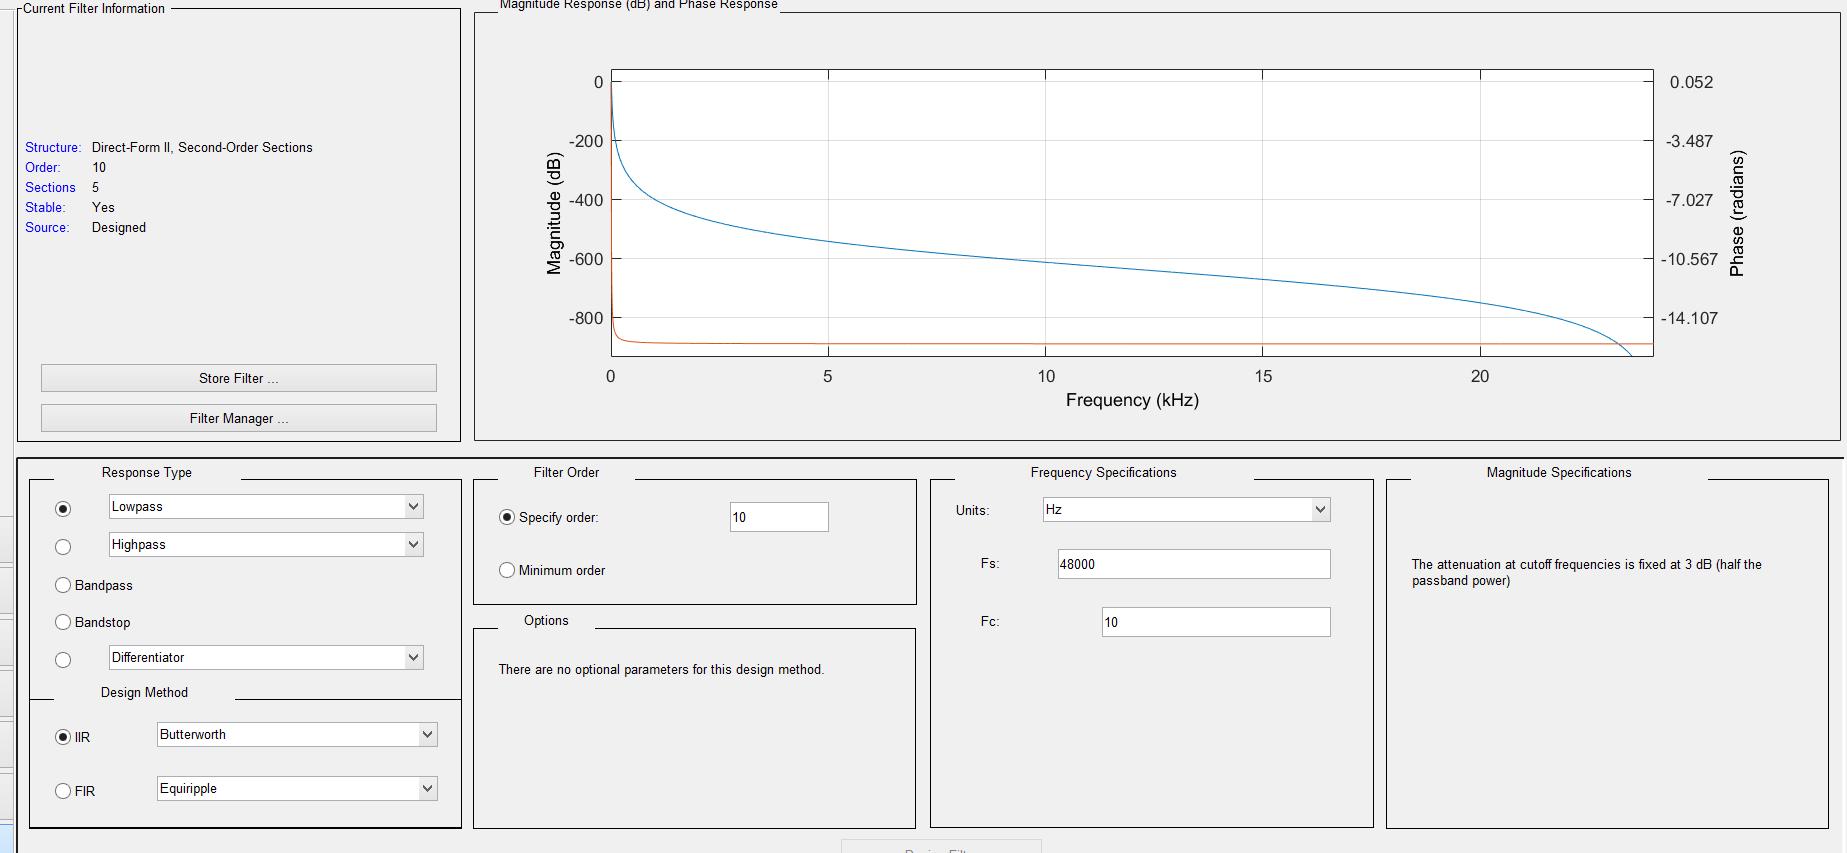
\includegraphics[width=150mm]{figures/FDATool.PNG}
%	\caption{Design af IIR lavpas filter i FDA tools i matlab}
%	\label{fig:FDAtools}
%\end{figure}

Filteret blev desginet med ønske i at skabe et IIR butterworth filter med en knækfrekvens på 10Hz og med en orden på 10. 
Da filteret var designet blev koefficenterne exporteret til et matlab-fil, der blev benyttet i funktionen IIR-lowpass filter.

Koden for IIR lavpas filter funktionen kan ses nedenuner:

\subsection{FIR-weight funktion}

Equalizeren blev kørt med forskellige signaler, hvor der blev eksperimenteret med forskellige vægtning af de enkelte Båndpas-filtre samt frekvensbåndet de dækkede. Efter at havde eksperimenteret med de forskellige frekvensbånd blev det bestemt, at de enkelte frekvensbånd skulle dække følgende frekvensområder, der alle ligger i det hørbare frekvensområde:
\begin{itemize}
	\item Bånd 1 -
	\item Bånd 2 -
	\item Bånd 3 -
	\item Bånd 4 -
	\item Bånd 5 -
\end{itemize}

\section{Resultat}
I dette afsnit fremstilles resultaterne af at køre Hørerapperatet på en række forskellige signaler.
